% !TeX program = xelatex
\documentclass[12pt]{extreport}
\usepackage{fontspec}
\setmainfont{TeX Gyre Termes}
\usepackage[a4paper,left=3cm,right=2.5cm,top=2.5cm,bottom=2.5cm]{geometry}
\usepackage{graphicx}
\usepackage{xcolor}
\usepackage{titlesec}
\usepackage{setspace}
\usepackage{amsmath}
\usepackage{array}
\usepackage{booktabs}
\usepackage{tabularx}
\usepackage{float}
\usepackage{caption}
\usepackage{subcaption}
\usepackage{enumitem}
\usepackage{algorithm}
\usepackage{algpseudocode}
\usepackage{listings}
\usepackage{tikz}
\usetikzlibrary{arrows.meta,positioning,shapes.geometric,fit}
\usepackage{xurl}
\usepackage{hyperref}
\usepackage{fancybox}

\definecolor{HUSTRed}{HTML}{B5121B}
\definecolor{HUSTDarkRed}{HTML}{841018}
\definecolor{SoftGray}{HTML}{F3F4F6}
\definecolor{MidGray}{HTML}{6B7280}

\graphicspath{{images/}{../docs/media/}}
\hypersetup{%
  colorlinks=true,
  linkcolor=HUSTDarkRed,
  citecolor=HUSTDarkRed,
  urlcolor=HUSTDarkRed,
  pdfauthor={Nhóm sinh viên thực hiện},
  pdftitle={Thiết kế nền tảng trò chơi nhúng trên STM32F429 với bộ dựng hình 3D phần mềm}
}

\setcounter{tocdepth}{2}
\setcounter{secnumdepth}{2}
\setstretch{1.17}
\setlength{\parindent}{1.25cm}
\setlength{\parskip}{0pt}
\setlength{\emergencystretch}{2em}
\widowpenalty=10000
\clubpenalty=10000
\displaywidowpenalty=10000

\titleformat{\chapter}[display]
  {\normalfont\bfseries}
  {\large\color{HUSTRed}\MakeUppercase{Chương~\thechapter}}
  {0.7ex}
  {\Huge\color{black}}
  [\vspace{0.5ex}{\color{HUSTRed}\titlerule}]
\titlespacing*{\chapter}{0pt}{15pt}{2.1ex}

\titleformat{\section}
  {\normalfont\Large\bfseries}
  {\color{HUSTRed}\thesection}
  {0.7em}
  {}
\titlespacing*{\section}{0pt}{1.9ex plus 0.3ex}{0.8ex}

\titleformat{\subsection}
  {\normalfont\large\bfseries}
  {\color{HUSTRed}\thesubsection}
  {0.7em}
  {}
\titlespacing*{\subsection}{0pt}{1.7ex plus 0.3ex}{0.7ex}

\renewcommand{\contentsname}{Mục lục}
\renewcommand{\figurename}{Hình}
\renewcommand{\tablename}{Bảng}
\renewcommand{\bibname}{Tài liệu tham khảo}
\floatname{algorithm}{Thuật toán}
\algrenewcommand\algorithmicrequire{\textbf{Đầu vào:}}
\algrenewcommand\algorithmicensure{\textbf{Đầu ra:}}
\algrenewcommand\algorithmicend{\textbf{kết thúc}}
\algrenewcommand\algorithmicdo{\textbf{thực hiện}}
\algrenewcommand\algorithmicwhile{\textbf{trong khi}}
\algrenewcommand\algorithmicfor{\textbf{với}}
\algrenewcommand\algorithmicif{\textbf{nếu}}
\algrenewcommand\algorithmicthen{\textbf{thì}}
\algrenewcommand\algorithmicelse{\textbf{ngược lại}}
\algrenewcommand\algorithmicreturn{\textbf{trả về}}

\captionsetup{font=small,labelfont=bf,labelsep=period}
\setlist[itemize]{leftmargin=1.8em,itemsep=0.35ex,topsep=0.6ex}
\setlist[enumerate]{leftmargin=2.1em,itemsep=0.35ex,topsep=0.6ex}
\renewcommand{\arraystretch}{1.18}
\newcolumntype{Y}{>{\raggedright\arraybackslash}X}
\newcolumntype{L}[1]{>{\raggedright\arraybackslash}p{#1}}
\newcolumntype{C}[1]{>{\centering\arraybackslash}p{#1}}

\lstset{%
  basicstyle=\ttfamily\small,
  columns=fullflexible,
  keepspaces=true,
  frame=single,
  rulecolor=\color{MidGray},
  backgroundcolor=\color{SoftGray},
  breaklines=true,
  showstringspaces=false,
  xleftmargin=0.4em,
  xrightmargin=0.4em
}

\tikzset{%
  block/.style={draw=HUSTRed,rounded corners=2pt,fill=SoftGray,
    align=center,minimum height=8mm,text width=27mm,font=\small},
  compactblock/.style={draw=HUSTRed,rounded corners=2pt,fill=SoftGray,
    align=center,minimum height=8mm,text width=23mm,font=\small},
  flow/.style={-{Latex[length=2mm]},thick,HUSTDarkRed},
  pendingflow/.style={-{Latex[length=2mm]},thick,dashed,MidGray}
}

\newcommand{\pendingvalue}[1]{%
  \textcolor{HUSTRed}{\bfseries CẦN #1}%
}
\newcommand{\figureplaceholder}[2][0.88\textwidth]{%
  \begin{center}
    \fcolorbox{HUSTRed}{SoftGray}{%
      \parbox[c][3.0cm][c]{#1}{\centering\color{HUSTDarkRed}\bfseries #2}%
    }
  \end{center}
}
\newcommand{\StudentRow}[2]{#1 & #2\\}


\newcommand{\UniversityName}{ĐẠI HỌC BÁCH KHOA HÀ NỘI}
\newcommand{\SchoolName}{Trường Công nghệ Thông tin và Truyền thông}
\newcommand{\ReportType}{BÁO CÁO BÀI TẬP LỚN MÔN HỌC}
\newcommand{\SemesterName}{Học kỳ 2025.2}
\newcommand{\ReportTitle}{Thiết kế nền tảng trò chơi nhúng trên STM32F429 với engine đồ họa 2D/3D dựa trên driver ILI9341}
\newcommand{\CourseName}{Hệ nhúng}
\newcommand{\CourseCode}{IT4210}
\newcommand{\InstructorName}{TS. Đỗ Công Thuần}
\newcommand{\ClassCode}{166152}
\newcommand{\ReportStudents}{%
  \StudentRow{Nguyễn Quý Đức}{20235682}%
  \StudentRow{Trần Đăng Sinh}{20235821}%
  \StudentRow{Nguyễn Hồng Dương}{20235693}%
  \StudentRow{Bùi Quang Phương}{20235809}%
}
\newcommand{\SubmissionPlace}{Hà Nội}
\newcommand{\SubmissionYear}{2026}

\begin{document}
\hypersetup{pageanchor=false}
\thispagestyle{empty}
\thisfancypage{\setlength{\fboxsep}{-5pt}\fbox}{}
\begin{center}
	{\fontsize{13pt}{1}\selectfont\textbf{\\ĐẠI HỌC BÁCH KHOA HÀ NỘI}}\\
	{\fontsize{13pt}{1}\selectfont\textbf{TRƯỜNG CÔNG NGHỆ THÔNG TIN VÀ TRUYỀN THÔNG}}\\
	\textbf{--------------------  o0o  ---------------------}\\[1cm]
	
\includegraphics[scale=0.1]{images/hust.jpg} \\[1.2cm]
	\textbf{{\LARGE Bài tập lớn kỳ 2025.2}}\\[1cm]
	\textbf{{\Large Thiết kế nền tảng trò chơi nhúng trên STM32F429\\với engine đồ họa 2D/3D dựa trên driver ILI9341}}\\[0.5cm]
	\textbf{{\large Học phần: Hệ nhúng}}\\
	\textbf{{\large Mã học phần: IT4210}}\\[0.5cm]
\end{center}

\begin{flushleft}
\begin{center}
\(
\begin{array}{lll}
\textbf{Giảng viên hướng dẫn:} & \textbf{TS. Đỗ Công Thuần} \\[0.2cm]
\text{Sinh viên thực hiện:} 
& \text{Nguyễn Quý Đức} & \text{20235682} \\
& \text{Trần Đăng Sinh} & \text{20235821} \\
& \text{Nguyễn Hồng Dương} & \text{20235693} \\
& \text{Bùi Quang Phương} & \text{20235809} \\
\text{Mã lớp:} &\text{166152}
\end{array}
\)
\end{center}
\end{flushleft}

\vspace*{\fill}
\begin{center}
\textbf{{\large Hà Nội - 2026}}\\
\end{center}
\newpage


\hypersetup{pageanchor=true}
\pagenumbering{roman}
\chapter*{Tóm tắt}
\addcontentsline{toc}{chapter}{Tóm tắt}

Báo cáo trình bày việc thiết kế một nền tảng trò chơi nhúng chạy trực tiếp trên vi điều khiển STM32F429ZIT6. Hệ thống tích hợp hai trò chơi có đặc điểm xử lý khác nhau: Stack 3D sử dụng bộ dựng hình ba chiều viết bằng C, còn Tetris sử dụng lưới hai chiều và cơ chế va chạm theo ô. Hình ảnh được xuất lên màn hình ILI9341 độ phân giải $320\times240$ qua SPI5. Người dùng điều khiển bằng nút PA0 hoặc bàn phím máy tính thông qua cầu nối Bluetooth Classic trên ESP32 và đường UART2 có DMA vòng.

Đóng góp kỹ thuật chính của đề tài là bộ dựng hình phần mềm phù hợp với giới hạn bộ nhớ của vi điều khiển. Pipeline thực hiện biến đổi World--View--Projection, loại mặt khuất, chiếu sáng phẳng, raster hóa scanline và kiểm tra độ sâu. Thay vì cấp phát framebuffer màu và độ sâu cho toàn màn hình, hệ thống xử lý theo hai dải, mỗi dải cao 120 dòng. Hai bộ đệm theo dải chiếm 153600 byte, bằng một nửa phương án toàn khung hình.

Mã nguồn đã bao gồm trình quản lý trạng thái, lớp ánh xạ đầu vào, hai trò chơi, driver màn hình và bộ dựng hình 2D/3D. ESP32 được cấp nguồn từ cổng USB OTG, còn dữ liệu điều khiển đi một chiều từ ESP32 đến STM32 qua UART2. Báo cáo đi kèm các hình ảnh thực nghiệm của cả hai trò chơi Stack 3D và Tetris chạy thực tế trên phần cứng nhằm xác minh hoạt động đúng đắn của hệ thống.
\noindent\textbf{Từ khóa:} STM32F429, hệ thống nhúng, đồ họa 3D phần mềm, Z-buffer, ILI9341, Tetris, Bluetooth SPP.
\clearpage

\begingroup
\footnotesize
\setstretch{1.0}
\tableofcontents
\endgroup
\clearpage

\pagenumbering{arabic}
\chapter{Tổng quan đề tài}
\label{chap:overview}

\section{Bối cảnh và động lực}

Các hệ thống nhúng hiện đại có đủ năng lực để thực hiện giao diện đồ họa và trò chơi tương tác mà không cần hệ điều hành. Đây là bài toán phù hợp để khảo sát đồng thời nhiều nội dung của kỹ thuật máy tính: cấu hình ngoại vi, quản lý bộ nhớ, xử lý thời gian thực, mô hình trạng thái, giao tiếp không dây và thuật toán đồ họa. STM32F429ZIT6 sử dụng lõi Arm Cortex-M4 có FPU, tích hợp 2 MB Flash và tổng cộng 256 KB SRAM theo tài liệu của nhà sản xuất~\cite{stm32datasheet}. Cấu hình này đủ để xây dựng một thiết bị chơi game nhỏ, nhưng vẫn buộc người thiết kế phải kiểm soát chặt bộ đệm đồ họa và chi phí tính toán.

Đề tài phát triển \textit{STM32 Retro Play}, một nền tảng gồm menu chọn trò chơi, Stack 3D và Tetris. Stack 3D đặt trọng tâm vào bộ dựng hình ba chiều viết hoàn toàn bằng C; Tetris đại diện cho trò chơi lưới hai chiều có luật va chạm, xoay khối và tính điểm. Hệ thống hiển thị trên LCD ILI9341 $320\times240$ và nhận lệnh từ nút vật lý hoặc cầu nối Bluetooth qua ESP32. Toàn bộ phân tích trong báo cáo bám theo mã nguồn của dự án.

\section{Bài toán cần giải quyết}

Một khung hình đầy đủ ở định dạng RGB565 cần $320\times240\times2=153600$ byte. Nếu bổ sung Z-buffer 16 bit cho dựng hình 3D, riêng hai framebuffer đã cần 307200 byte, lớn hơn vùng RAM 192 KiB mà linker hiện dành cho dữ liệu thông thường. Bên cạnh giới hạn bộ nhớ, hệ thống còn phải xử lý luật của hai trò chơi, cập nhật theo thời gian, dựng giao diện và truyền số lượng lớn điểm ảnh qua SPI mà không dùng hệ điều hành.

Bài toán được chia thành bốn nhóm:
\begin{itemize}
  \item xây dựng kiến trúc mô-đun để menu và các trò chơi dùng chung đầu vào, hiển thị và vòng lặp chính;
  \item hiện thực bộ dựng hình 3D có phép chiếu phối cảnh, loại mặt khuất, chiếu sáng phẳng và kiểm tra độ sâu;
  \item hiện thực luật Stack 3D và Tetris với trạng thái trò chơi rõ ràng;
  \item tích hợp đường điều khiển từ PC qua Bluetooth Classic, ESP32 và UART2 trên STM32.
\end{itemize}

\section{Mục tiêu}

Mục tiêu tổng quát là tạo một nguyên mẫu nền tảng trò chơi nhúng chạy trực tiếp trên STM32F429 và có cấu trúc đủ rõ để bổ sung trò chơi mới. Các mục tiêu cụ thể gồm:
\begin{enumerate}
  \item Hiển thị menu và hai trò chơi trên LCD ILI9341 ở chế độ ngang;
  \item Ánh xạ ký tự đầu vào thành hành động logic dùng chung cho menu, Stack 3D và Tetris;
  \item Duy trì luật chơi, điểm số, màn hình kết thúc và thao tác khởi động lại;
  \item Ghi nhận trung thực phần đã hiện thực, phần mới cấu hình và phần chưa có số đo thực nghiệm.
\end{enumerate}

\section{Phạm vi và giới hạn}

Phạm vi báo cáo bao gồm mã ứng dụng trong \texttt{Core/}, cầu nối trong \texttt{Others/}, cấu hình STM32CubeMX và các thư viện STM32CubeF4 được repository sử dụng.

\section{Yêu cầu hệ thống}

Bảng~\ref{tab:requirements} tổng hợp các yêu cầu có thể đối chiếu trực tiếp với mã nguồn và bằng chứng trong repository.

\begin{table}[H]
\centering
\small
\caption{Yêu cầu chính của nền tảng}
\label{tab:requirements}
\begin{tabularx}{\textwidth}{@{}p{0.16\textwidth}Y Y@{}}
\toprule
\textbf{Nhóm} & \textbf{Yêu cầu} & \textbf{Tiêu chí đối chiếu} \\
\midrule
Hiển thị & Xuất giao diện $320\times240$ ở định dạng RGB565 & Có driver ILI9341 và truyền khối điểm ảnh qua SPI5 \\
Đầu vào & Dùng chung hành động lên, xuống, trái, phải và chọn & Mọi ký tự đi qua \texttt{InputManager\_MapCharacter} \\
Stack 3D & Cắt phần thừa, tạo khối rơi và tăng tốc theo điểm & Kích thước khối mới bằng phần giao nhau với khối đỉnh \\
Tetris & Hỗ trợ bảy tetromino, xoay, xóa dòng, điểm và cấp độ & Lưới $20\times10$, kiểm tra va chạm trước mọi dịch chuyển \\
Bộ nhớ & Không cấp phát đồng thời framebuffer màu và độ sâu toàn màn hình & Dựng theo hai chunk, mỗi chunk cao 120 dòng \\
Tính đúng đắn & Không tuyên bố kết quả chưa có bằng chứng & Chỉ số chưa đo và ảnh thiếu phải có nhãn chờ \\
\bottomrule
\end{tabularx}
\end{table}

\subsection{Yêu cầu chức năng}

Hệ thống phải khởi tạo được màn hình ILI9341 ở chế độ ngang, hiển thị menu lựa chọn và chạy được hai trò chơi Stack 3D và Tetris. Người dùng phải điều hướng được menu, thực hiện các thao tác đặc trưng của từng trò chơi, xem điểm số, nhận biết trạng thái game over, khởi động lại trò chơi hoặc quay về menu. Lệnh điều khiển được tiếp nhận từ nút PA0 và từ bàn phím PC thông qua cầu nối Bluetooth Classic trên ESP32. Dữ liệu từ ESP32 được chuyển tới STM32 bằng UART2 và chuẩn hóa thành tập hành động dùng chung trước khi chuyển cho menu hoặc game.

\subsection{Yêu cầu phi chức năng}

Nguyên mẫu phải hoạt động ổn định trên STM32F429ZIT6 mà không cần RTOS, không vượt vùng RAM do linker cấp cho dữ liệu thông thường, và không cấp phát động trong vòng lặp dựng hình. Thiết kế phần mềm cần có ranh giới mô-đun rõ ràng để có thể bổ sung trò chơi mới. Hệ thống ghép nối phải đủ chắc chắn cho việc trình diễn trên bàn; dây nguồn và tín hiệu cần được cố định, không để chân tín hiệu ở trạng thái không xác định. Giao diện phải đọc được trên màn hình $320\times240$, phản hồi đầu vào trong quá trình truyền khung hình, và tài liệu phải cho phép người khác build, flash và chạy lại project.

\chapter{Cơ sở kỹ thuật và kiến trúc hệ thống}
\label{chap:architecture}

\section{Nền tảng phần cứng}

Vi điều khiển trung tâm là STM32F429ZIT6. Dòng STM32F429 cung cấp lõi Cortex-M4 với FPU, nhiều ngoại vi truyền thông và USB OTG; chi tiết thanh ghi, kiến trúc bus và ngoại vi được mô tả trong RM0090~\cite{stm32datasheet,rm0090}. Project cấu hình HSE 8 MHz và PLL để chạy lõi ở 168 MHz. Mức này thấp hơn giới hạn tối đa của linh kiện nhưng cần vì bắt buộc cấu hình xung cấp cho USB OTG ở 48MHz.

Màn hình ILI9341 được điều khiển bằng SPI5 ở chế độ master. Dữ liệu điểm ảnh dùng RGB565, nghĩa là mỗi điểm ảnh chiếm 16 bit.

\begin{table}[H]
\centering
\small
\caption{Cấu hình ngoại vi chính}
\label{tab:hardware}
\begin{tabularx}{\textwidth}{@{}L{0.20\textwidth}L{0.27\textwidth}Y@{}}
\toprule
\textbf{Khối} & \textbf{Cấu hình} & \textbf{Vai trò} \\
\midrule
STM32F429ZIT6 & HSE 8 MHz, SYSCLK 168 MHz & Chạy vòng lặp, luật game và dựng hình \\
ILI9341 & $320\times240$, RGB565; SPI5 42 Mbit/s; PF7/PF9 & Hiển thị menu, Stack 3D và Tetris \\
USART2 RX & 921600 baud; PA3; DMA1 Stream 5 vòng & Nhận dữ liệu điều khiển từ ESP32 vào STM32 \\
Nút người dùng & PA0, EXTI cạnh lên, debounce 50 ms & Phát hành động chọn \\
USB OTG FS & PC4 điều khiển nguồn VBUS & Cấp nguồn cho ESP32; không tham gia truyền dữ liệu game \\
\bottomrule
\end{tabularx}
\end{table}

Các chân điều khiển LCD được khai báo trong driver: CS tại PC2, D/C tại PD13 và Reset tại PD12. ESP32 dùng UART2 TX trên chân GPIO17 để nối tới PA3 (USART2 RX) của STM32; GPIO16 được cấu hình RX trên ESP32 nhưng luồng điều khiển của phiên bản hiện tại chỉ đi một chiều. Hai board phải nối chung mass. SPI5 TX sử dụng DMA2 Stream 4 khi gửi các khối điểm ảnh tới LCD.

\section{Đường điều khiển không dây}

Máy tính chạy \texttt{Others/bluetooth.py} để đọc phím tức thời và gửi byte qua socket RFCOMM\@. Script tự tìm thiết bị \texttt{ESP32\_Bridge\_Logger} trong Windows Registry, sau đó kết nối Serial Port Profile trên kênh 1. ESP32 dùng \texttt{BluetoothSerial} để nhận các byte Bluetooth Classic và chuyển nguyên trạng sang STM32 qua UART2 ở 921600 baud. UART2 là đường dữ liệu một chiều từ ESP32 đến STM32 trong hệ thống hiện tại.

Trên STM32, module \texttt{espuart} khởi động DMA nhận vòng 256 byte. Hàm polling so sánh chỉ số đọc với vị trí ghi hiện tại của DMA, lấy từng byte và gọi callback. Callback chuyển ký tự sang \texttt{InputAction\_t}; nhờ đó, game không phụ thuộc vào nguồn nhập cụ thể. Đường truyền hiện tại là Bluetooth SPP - ESP32 - UART2, không phải I2C.

\section{Kiến trúc tổng thể}

Hình~\ref{fig:system-architecture} mô tả luồng dữ liệu và nguồn của nguyên mẫu. Cổng USB OTG chỉ được dùng để cấp nguồn cho ESP32, không phải một đường nhập liệu. Dữ liệu điều khiển đi từ PC qua Bluetooth SPP đến ESP32, sau đó được ESP32 chuyển sang STM32 qua UART2 RX và DMA vòng.

\begin{figure}[H]
\centering
\begin{tikzpicture}[node distance=7mm and 8mm]
  \node[block] (pc) {PC\\Python controller};
  \node[block, right=of pc] (bt) {Bluetooth SPP\\ESP32};
  \node[block, right=of bt] (uart) {UART2 RX\\DMA vòng};
  \node[block, right=of uart] (input) {InputManager\\hành động logic};
  \node[block, below=10mm of input] (state) {AppState\\Manager\\menu và game};
  \node[block, left=of state] (games) {Stack 3D\\Tetris};
  \node[block, left=of games] (gfx) {Graphics 2D/3D\\chunk + Z-buffer};
  \node[block, left=of gfx] (lcd) {SPI5\\ILI9341};
  \node[compactblock, above=8mm of bt] (usb) {USB OTG\\cấp nguồn ESP32};
  \node[compactblock, above=8mm of input] (button) {Nút PA0\\EXTI};

  \draw[flow] (pc) -- (bt);
  \draw[flow] (bt) -- (uart);
  \draw[flow] (uart) -- (input);
  \draw[flow] (input) -- (state);
  \draw[flow] (state) -- (games);
  \draw[flow] (games) -- (gfx);
  \draw[flow] (gfx) -- (lcd);
  \draw[flow] (button) -- (input);
  \draw[flow] (usb) -- node[right, font=\scriptsize] {nguồn} (bt);
\end{tikzpicture}
\caption{Kiến trúc dữ liệu và điều khiển của hệ thống}
\label{fig:system-architecture}
\end{figure}

\section{Tổ chức phần mềm}

Phần ứng dụng được chia theo trách nhiệm như Bảng~\ref{tab:modules}.

\begin{table}[H]
\centering
\caption{Các mô-đun phần mềm chính}
\label{tab:modules}
\small
\begin{tabularx}{\textwidth}{@{}p{0.24\textwidth}Y Y@{}}
\toprule
\textbf{Mô-đun} & \textbf{Trách nhiệm} & \textbf{Giao diện chính} \\
\midrule
\texttt{main.c} & Khởi tạo ngoại vi, lấy $\Delta t$, đọc sự kiện nút và gọi vòng lặp ứng dụng & \texttt{main}, callback EXTI/UART \\
\texttt{input\_manager} & Chuẩn hóa ký tự thành hành động logic & \texttt{InputManager\_MapCharacter} \\
\texttt{app\_state\_manager} & Quản lý menu, game hiện tại, con trỏ và màn hình game over & Init, Update, Render, HandleAction \\
\texttt{stack\_game} & Luật Stack, vật lý mảnh rơi, camera và đối tượng render & Init, Update, HandlePress, Render \\
\texttt{tetris\_game} & Lưới, tetromino, va chạm, xóa dòng, điểm và giao diện & Init, Update, HandleAction, Render \\
\texttt{graphics\_3d} & Toán vector/ma trận, rasterizer, Z-buffer, chunk và overlay & \texttt{GFX3D\_RenderObjects} \\
Driver ILI9341 & Gửi lệnh, màu và khối điểm ảnh tới LCD & Init, SetAddress, SendPixelBuffer \\
\bottomrule
\end{tabularx}
\end{table}

\section{Luồng thực thi}

Sau khi HAL và ngoại vi được khởi tạo, chương trình cấu hình nguồn cho ESP32, màn hình, UART2 RX DMA và state manager. Mỗi vòng lặp polling UART2, lấy các lần nhấn PA0 trong vùng bảo vệ ngắt, tính $\Delta t$, cập nhật state rồi render toàn màn hình. Kiến trúc không dùng RTOS; mọi phần việc chạy tuần tự trong vòng lặp chính, còn DMA và ngắt chỉ đảm nhiệm tiếp nhận dữ liệu hoặc ghi nhận sự kiện ngắn.

\chapter{Thiết kế và hiện thực}
\label{chap:implementation}

\section{Quản lý trạng thái ứng dụng}

Ứng dụng có ba trạng thái cấp cao: menu chính, Stack 3D và Tetris. Mảng cấu hình \texttt{game\_screens} lưu tên, hitbox và các con trỏ hàm của từng trò chơi. State manager chỉ gọi qua giao diện \texttt{start}, \texttt{restart}, \texttt{update}, \texttt{render}, \texttt{handle\_play\_action} và \texttt{is\_game\_over}. Cách tổ chức này cho phép menu xử lý hai game theo cùng một luồng mà không cần kiểm tra loại game tại nhiều vị trí.

Trong menu, WASD dịch con trỏ 15 điểm ảnh theo mỗi lệnh. Khi nhận hành động chọn, state manager kiểm tra con trỏ có nằm trong hitbox của thẻ Stack hoặc Tetris hay không. Trong trạng thái chơi, lệnh được chuyển cho game hiện tại. Khi game over, con trỏ xuất hiện lại để người dùng chọn \texttt{RESTART} hoặc \texttt{MENU}.

Nút PA0 chỉ tạo \texttt{INPUT\_ACTION\_SELECT}. Vì vị trí con trỏ khởi tạo $(160,120)$ nằm giữa hai thẻ menu, riêng nút này chưa đủ để chọn game từ lúc khởi động. Người dùng cần nguồn lệnh có các hướng di chuyển, hiện là cầu nối Bluetooth.

\section{Chuẩn hóa đầu vào}

Kiểu \texttt{InputAction\_t} gồm sáu giá trị: không hành động, lên, xuống, trái, phải và chọn. Bảng~\ref{tab:controls} cho thấy ánh xạ thực tế trong mã nguồn. Enter và các mã phím mũi tên nhiều byte chưa được xử lý.

\begin{table}[H]
  \centering
  \caption{Ánh xạ đầu vào của phiên bản hiện tại}
  \label{tab:controls}
  \begin{tabularx}{0.78\textwidth}{@{}C{0.18\textwidth}Y Y@{}}
    \toprule
    \textbf{Ký tự}        & \textbf{Hành động} & \textbf{Cách dùng}                         \\
    \midrule
    \texttt{W}/\texttt{w} & Lên                & Di chuyển con trỏ hoặc xoay tetromino      \\
    \texttt{S}/\texttt{s} & Xuống              & Di chuyển con trỏ hoặc soft drop           \\
    \texttt{A}/\texttt{a} & Trái               & Di chuyển con trỏ hoặc khối Tetris         \\
    \texttt{D}/\texttt{d} & Phải               & Di chuyển con trỏ hoặc khối Tetris         \\
    \texttt{1}, Space     & Chọn               & Chọn menu, đặt khối Stack hoặc hard drop   \\
    PA0                   & Chọn               & Tạo cùng hành động chọn sau debounce 50 ms \\
    \bottomrule
  \end{tabularx}
\end{table}

\section{Pipeline dựng hình 3D}

Bộ dựng hình không dùng thư viện đồ họa ngoài. Mỗi đối tượng gồm một mesh, ma trận World và màu RGB565. Với đỉnh $\mathbf{p}$, tọa độ clip được tính theo
\begin{equation}
  \mathbf{p}_{clip}=\mathbf{P}\mathbf{V}\mathbf{W}\mathbf{p},
  \label{eq:mvp}
\end{equation}
trong đó $\mathbf{W}$ biến đổi mô hình, $\mathbf{V}$ biểu diễn camera và $\mathbf{P}$ là phép chiếu phối cảnh. Sau phép chia cho thành phần $w$, tọa độ chuẩn hóa được ánh xạ sang màn hình $320\times240$. Giá trị $1/w$ được nội suy và lượng tử hóa về 16 bit để so sánh độ sâu.

Với mỗi tam giác, renderer tính diện tích có hướng trong không gian màn hình. Tam giác có diện tích không dương bị loại như mặt quay lưng. Pháp tuyến trong không gian thế giới được tính bằng tích có hướng của hai cạnh. Cường độ sáng là tích vô hướng với vector ánh sáng, sau đó kết hợp thành phần ambient 0,55 để tạo màu phẳng trên mỗi mặt.

\begin{figure}[H]
  \centering
  \resizebox{\textwidth}{!}{%
    \begin{tikzpicture}[node distance=6mm]
      \node[compactblock] (object) {Đối tượng\\mesh + World};
      \node[compactblock, right=of object] (mvp) {World--View--Projection};
      \node[compactblock, right=of mvp] (project) {Chiếu đỉnh\\về màn hình};
      \node[compactblock, right=of project] (cull) {Loại mặt\\quay lưng};
      \node[compactblock, right=of cull] (light) {Chiếu sáng\\phẳng};
      \node[compactblock, right=of light] (raster) {Scanline +\\Z-buffer};
      \node[compactblock, right=of raster] (overlay) {HUD/overlay\\theo chunk};
      \node[compactblock, right=of overlay] (output) {RGB565\\SPI5 - LCD};
      \draw[flow] (object) -- (mvp);
      \draw[flow] (mvp) -- (project);
      \draw[flow] (project) -- (cull);
      \draw[flow] (cull) -- (light);
      \draw[flow] (light) -- (raster);
      \draw[flow] (raster) -- (overlay);
      \draw[flow] (overlay) -- (output);
    \end{tikzpicture}%
  }
  \caption{Các bước dựng một khung hình 3D}
  \label{fig:render-pipeline}
\end{figure}

Tam giác được sắp theo tung độ rồi chia thành tam giác đáy phẳng hoặc đỉnh phẳng. Mỗi scanline nội suy biên trái, biên phải và độ sâu. Pixel chỉ ghi màu khi giá trị độ sâu mới lớn hơn giá trị đang lưu.

\begin{algorithm}[H]
  \caption{Dựng nhiều đối tượng theo từng chunk}
  \label{alg:chunk-render}
  \begin{algorithmic}[1]
    \Require Danh sách đối tượng, ma trận View, Projection
    \Ensure Hai dải điểm ảnh được gửi tuần tự tới LCD
    \For{$chunk \gets 0$ đến $1$}
    \State Xóa color buffer và Z-buffer của 120 dòng hiện tại
    \State Vẽ nền của chunk
    \For{mỗi đối tượng}
    \State Tính $MVP=P\times V\times W$ và chiếu các đỉnh
    \For{mỗi mặt tam giác giao với chunk}
    \If{mặt hướng về camera}
    \State Tính màu theo pháp tuyến và nguồn sáng
    \State Raster hóa scanline, chỉ ghi pixel vượt kiểm tra độ sâu
    \EndIf
    \EndFor
    \EndFor
    \State Vẽ HUD hoặc con trỏ lên color buffer
    \State Đổi thứ tự byte RGB565 và truyền chunk qua SPI5
    \EndFor
  \end{algorithmic}
\end{algorithm}

\section{Tối ưu bộ nhớ theo chunk}

Hai mảng tĩnh \texttt{chunk\_color\_buffer} và \texttt{chunk\_z\_buffer} đều có $320\times120$ phần tử 16 bit. Tổng dung lượng là
\begin{equation}
  M_{chunk}=2\times320\times120\times2=153600\ \text{byte}=150\ \text{KiB}.
  \label{eq:chunk-memory}
\end{equation}
Nếu lưu cả màu và độ sâu cho toàn màn hình, dung lượng tương ứng là
\begin{equation}
  M_{full}=2\times320\times240\times2=307200\ \text{byte}=300\ \text{KiB}.
  \label{eq:full-memory}
\end{equation}
Vùng RAM thông thường dài 192 KiB và CCMRAM 64 KiB. Hai framebuffer toàn màn hình vượt riêng vùng RAM 192 KiB, trong khi phương án chunk giảm một nửa dung lượng. Thiết kế hiện tại vì thế để lại ít biên RAM cho middleware và trạng thái game.

Mỗi chunk được truyền xuống LCD thông qua kênh DMA2 Stream 4 của SPI5 ở chế độ không chặn (\texttt{HAL\_SPI\_Transmit\_DMA}). Trong thời gian chờ DMA hoàn thành việc truyền dữ liệu màn hình, CPU liên tục gọi hàm thăm dò \texttt{espuart\_poll()} để tiếp nhận và xử lý các sự kiện điều khiển từ ESP32 qua UART2. Cách xen kẽ này giảm thời gian đầu vào phải chờ so với truyền SPI chặn, nhưng project hiện chưa có phép đo độ trễ đầu vào bằng thiết bị chuyên dụng.

\section{Thiết kế Stack 3D}

Trạng thái Stack chứa tối đa 20 khối đã đặt, một khối đang di chuyển và bốn mảnh rơi. Mỗi lượt đổi trục chuyển động giữa $X$ và $Z$. Vận tốc tăng theo điểm số người chơi:
\begin{equation}
  v=\min(1.2+0.08\times score,\ 3.0)\ \text{đơn vị/s}.
\end{equation}
Khối hoạt động đi lại trong khoảng $\pm2.5$ quanh tâm khối đỉnh. Khi người chơi nhấn chọn, thuật toán lấy khoảng giao nhau trên trục hiện tại:
\begin{equation}
  overlap=\min(a_{\max},t_{\max})-\max(a_{\min},t_{\min}),
  \label{eq:stack-overlap}
\end{equation}
với $a$ (active) là khối hoạt động và $t$ (top) là khối đỉnh. Nếu \textit{overlap} không dương, game chuyển sang game over. Ngược lại, phần giao trở thành khối mới; phần thừa trở thành mảnh rơi có gia tốc $4.5$ đơn vị/s$^2$. Camera nội suy về vị trí khối đỉnh để theo dõi tháp khi chiều cao tăng.

Renderer tạo một cube mesh dùng chung, sau đó thay đổi ma trận tịnh tiến và tỉ lệ cho từng khối. Các đối tượng cùng chia sẻ Z-buffer theo chunk, vì vậy mảnh rơi và các tầng tháp che khuất nhau theo độ sâu thay vì phụ thuộc thứ tự vẽ.

\begin{figure}[H]
\centering
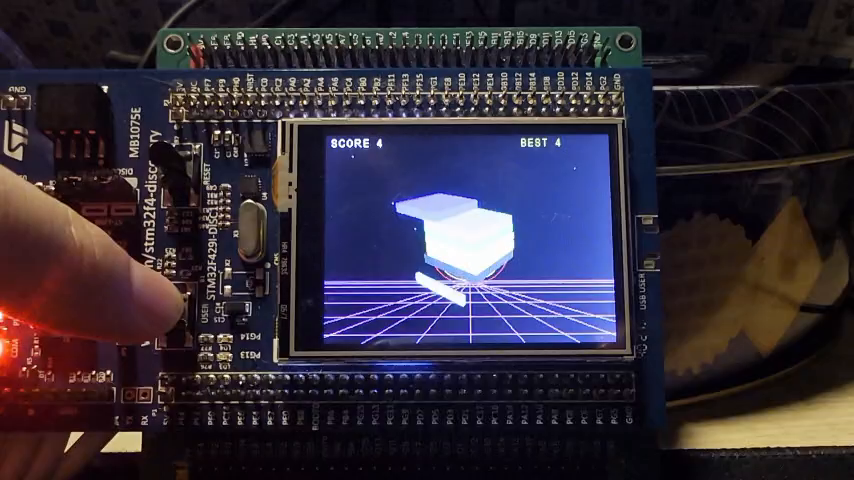
\includegraphics[width=0.6\textwidth]{stack-gameplay-frame.png}
\caption{Giao diện trò chơi Stack 3D với góc nhìn phối cảnh và bộ đệm độ sâu Z-buffer}
\label{fig:stack-gameplay}
\end{figure}



\section{Thiết kế Tetris}

Tetris dùng lưới $20\times10$ phần tử RGB565. Bảy tetromino được mô tả bởi bốn trạng thái xoay, mỗi trạng thái gồm bốn tọa độ tương đối. Trước mọi thao tác, \texttt{CheckCollision} kiểm tra biên trái/phải, đáy và các ô đã khóa. Khi xoay không hợp lệ tại chỗ, chương trình thử dịch một ô sang trái rồi một ô sang phải; đây là wall kick đơn giản trong Tetris cổ điển.

Khi khối chạm đáy hoặc khối đã khóa, bốn ô được ghi vào lưới. Thuật toán quét từ hàng cuối lên trên; với hàng đầy, các hàng phía trên dịch xuống và chỉ số hàng được kiểm tra lại. Điểm cho một đến bốn dòng lần lượt là 40, 100, 300 và 1200, nhân với $level+1$. Cứ mười dòng, cấp độ tăng và khoảng rơi tự động giảm từ 0,80 giây xuống tối thiểu 0,08 giây.

\begin{figure}[H]
\centering
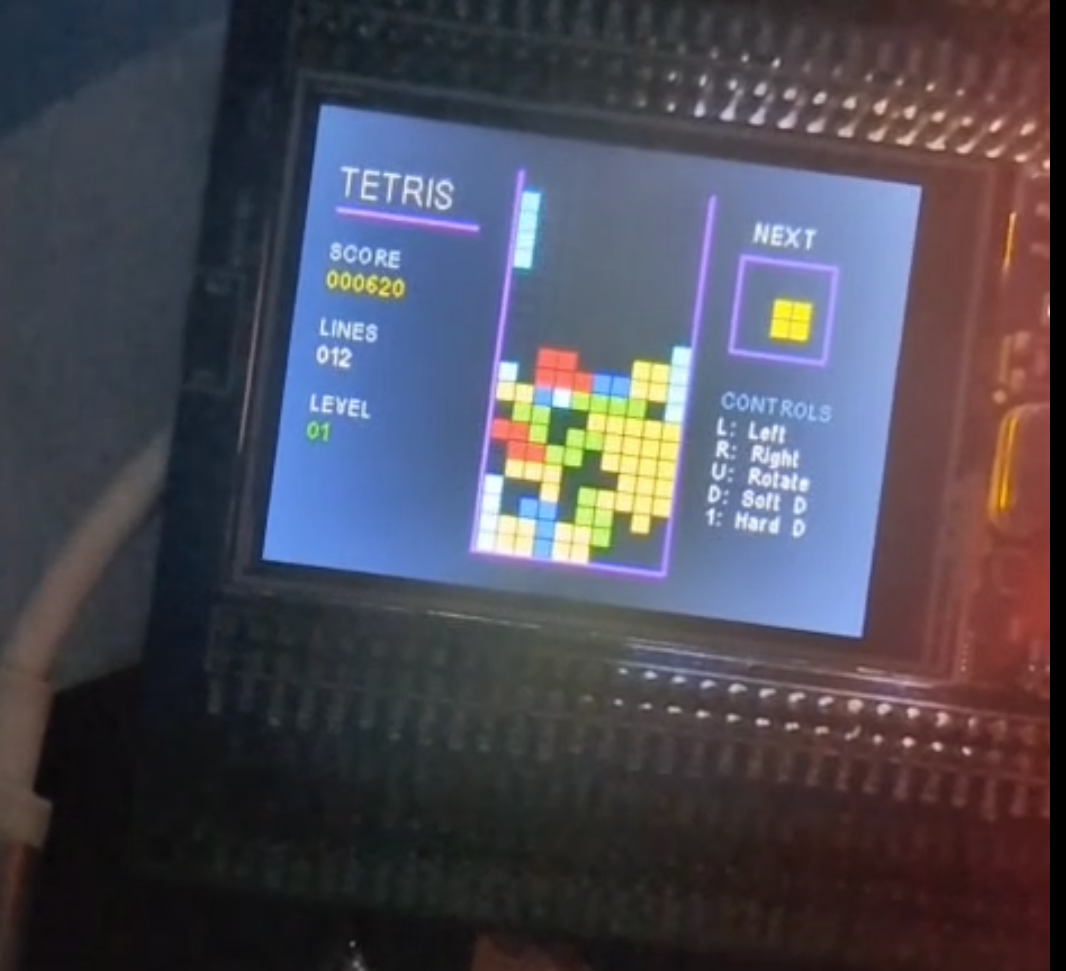
\includegraphics[width=0.6\textwidth]{tetris-gameplay.png}
\caption{Giao diện trò chơi Tetris hiển thị trên màn hình ILI9341}
\label{fig:tetris-gameplay}
\end{figure}



\section{Tích hợp hiển thị và giao diện}

Menu và Tetris vẽ trực tiếp vào color buffer theo chunk. Stack 3D dùng overlay callback để ghép điểm số, best score và hộp game over sau bước rasterization. Sau khi hoàn thành chunk, hàm gửi buffer đổi byte của từng giá trị RGB565 để byte cao được truyền trước, đặt vùng địa chỉ LCD rồi gửi dữ liệu qua SPI5.

\chapter{Cài đặt, kết quả và đánh giá}
\label{chap:deployment}

\section{Môi trường phát triển và cách cài đặt}

Mã nguồn project được lưu tại \url{https://github.com/nqd2/stm32-simple-gameboy}. File cấu hình \path{stm3d.ioc} được tạo cho STM32F429ZITx bằng STM32CubeMX 6.18.0; toolchain đích là STM32CubeIDE. Firmware ESP32 sử dụng Arduino core for ESP32 và thư viện \path{BluetoothSerial}. Chương trình điều khiển trên PC sử dụng Python 3. Các version không được khóa trong repository phải được kiểm tra lại trên máy build nếu cần tái tạo chính xác môi trường.

Quy trình cài đặt gồm:
\begin{enumerate}
  \item Clone repository và import project \path{stm3d} vào STM32CubeIDE bằng chức năng \textit{Existing Projects into Workspace};
  \item Mở \path{stm3d.ioc}, kiểm tra target STM32F429ZITx, sinh lại mã nếu thay đổi cấu hình, sau đó build cấu hình Debug;
  \item Kết nối ST-LINK, flash firmware lên STM32F429 và nối LCD ILI9341 theo bảng chân trong Chương~\ref{chap:architecture};
  \item Build và nạp \path{Others/esp32sketch/esp32sketch.ino} lên ESP32, nối GPIO17 của ESP32 với PA3 của STM32 và nối chung GND;
  \item Pair thiết bị \path{ESP32_Bridge_Logger} với PC, cài Python và chạy lệnh \path{python Others/bluetooth.py} để gửi phím.
\end{enumerate}

\section{Các mô-đun cài đặt chính}

Phần cài đặt được chia thành bốn lớp. Lớp phần cứng gồm HAL, cấu hình clock, GPIO, DMA, SPI5 và USART2. Lớp driver gồm ILI9341, font, UART nhận vòng và ánh xạ đầu vào. Lớp nền tảng gồm đồ họa 2D/3D và trình quản lý trạng thái. Lớp ứng dụng gồm menu, Stack 3D và Tetris. Phía ngoài STM32 có ESP32 làm cầu nối byte Bluetooth--UART và script Python bắt phím trên PC. Ranh giới này giúp logic game chỉ phụ thuộc \texttt{InputAction\_t} và các hàm render, không phụ thuộc trực tiếp vào Bluetooth hoặc thanh ghi ngoại vi.

\section{Phân công và mức độ đóng góp}

Nhóm thống nhất mức đóng góp tổng là 25\% cho mỗi thành viên. Bảng~\ref{tab:contributions} tính trên 13 commit kỹ thuật trước commit bổ sung tài liệu báo cáo. Số commit chỉ phản ánh cách chia lịch sử theo phần việc chính; một commit có thể chứa mã sinh tự động hoặc thay đổi giao thoa giữa nhiều mô-đun nên không được dùng riêng lẻ để suy ra khối lượng công việc.

\begin{table}[H]
\centering
\scriptsize
\caption{Phân công và đóng góp của thành viên}
\label{tab:contributions}
\begin{tabularx}{\textwidth}{@{}L{0.18\textwidth}L{0.13\textwidth}Y C{0.09\textwidth}C{0.09\textwidth}@{}}
\toprule
\textbf{Thành viên} & \textbf{GitHub} & \textbf{Nhiệm vụ chính} & \textbf{Commit} & \textbf{Đóng góp} \\
\midrule
Nguyễn Quý Đức & \texttt{nqd2} & Xây dựng engine đồ họa 2D/3D từ driver ILI9341; tích hợp SPI DMA và nền tảng hiển thị & 5 & 25\% \\
Bùi Quang Phương & \texttt{F3ust} & Điều khiển Bluetooth PC--ESP32--STM32; chuẩn hóa đầu vào và menu chọn hai game & 3 & 25\% \\
Trần Đăng Sinh & \texttt{MikoUwU24} & Thiết kế, cài đặt và chuẩn bị demo trò chơi Stack 3D & 2 & 25\% \\
Nguyễn Hồng Dương & \texttt{BlackHoleHiHi} & Thiết kế và cài đặt trò chơi Tetris & 3 & 25\% \\
\bottomrule
\end{tabularx}
\end{table}

Email dùng để nhận diện commit lần lượt là \nolinkurl{nguyenquyduc_hsgs20@hus.edu.vn}, \nolinkurl{hd3876536@gmail.com}, \nolinkurl{ctan4991@gmail.com} và \nolinkurl{nguyenhongduong01092005@gmail.com}.

\section{Kết quả và bằng chứng demo}

Nguyên mẫu đã hiển thị được menu và hai trò chơi trên LCD ILI9341. Stack 3D có chuyển động luân phiên theo hai trục, cắt phần thừa, mảnh rơi, điểm số và camera theo tháp. Tetris có bảy tetromino, xoay, dịch chuyển, soft drop, hard drop, xóa dòng, điểm và cấp độ. Hai game dùng chung menu, đầu vào và luồng game over/restart.

Bằng chứng demo được lưu cùng repository để link còn hiệu lực trong suốt học kỳ:
\begin{itemize}
  \item Video Stack 3D: \href{https://github.com/nqd2/stm32-simple-gameboy/blob/main/docs/media/stack-3d-demo.mp4}{docs/media/stack-3d-demo.mp4};
  \item Ảnh Stack 3D: \href{https://github.com/nqd2/stm32-simple-gameboy/blob/main/docs/media/stack-3d-demo-cover.png}{stack-3d-demo-cover.png};
  \item Ảnh Tetris: \href{https://github.com/nqd2/stm32-simple-gameboy/blob/main/docs/media/tetris-demo-cover.png}{tetris-demo-cover.png}.
\end{itemize}

\section{Đánh giá}

\begin{table}[H]
\centering
\small
\caption{Đối chiếu kết quả với yêu cầu}
\label{tab:evaluation}
\begin{tabularx}{\textwidth}{@{}L{0.26\textwidth}C{0.16\textwidth}Y@{}}
\toprule
\textbf{Yêu cầu} & \textbf{Trạng thái} & \textbf{Bằng chứng/giới hạn} \\
\midrule
Menu và hai trò chơi & Đạt & Mã nguồn, ảnh và video demo trong repository \\
Đồ họa 2D/3D trên ILI9341 & Đạt & Renderer, Z-buffer theo chunk và SPI5 DMA \\
Điều khiển không dây & Đạt & PC--Bluetooth SPP--ESP32--UART2 DMA \\
Phản hồi thời gian thực & Đạt một phần & Có polling UART trong lúc SPI DMA; chưa đo định lượng input latency và FPS \\
Độ hoàn thiện cơ khí & Đạt mức nguyên mẫu & Mạch ghép nối phục vụ demo; chưa có PCB/vỏ bảo vệ riêng \\
Khả năng mở rộng & Đạt & Giao diện game và \texttt{InputAction\_t} tách khỏi nguồn nhập cụ thể \\
\bottomrule
\end{tabularx}
\end{table}

Ưu điểm chính là kiến trúc mô-đun, renderer không phụ thuộc thư viện đồ họa ngoài, tiết kiệm RAM bằng chunk và hỗ trợ hai nguồn điều khiển. Hạn chế gồm chưa đo FPS/input latency bằng thiết bị ngoài, chỉ có một nút vật lý cho hành động chọn, giao tiếp Bluetooth phụ thuộc ESP32 và PC, chưa có âm thanh, PCB hoặc vỏ hoàn thiện.

\section{AI-assisted disclaimer}

Nhóm \textbf{có sử dụng} công cụ AI để hỗ trợ rà soát cấu trúc repository, đối chiếu báo cáo với mã nguồn, biên tập LaTeX và phát hiện mô tả không còn đúng sau khi project chuyển từ I2C sang UART2. Các prompt chính yêu cầu: phân tích yêu cầu báo cáo cuối kỳ; xác định module phần cứng/phần mềm từ repository; lập bảng phân công và commit; kiểm tra tính nhất quán của thông số SPI, UART, DMA; và đề xuất cách trình bày kết quả, giới hạn. Nhóm chịu trách nhiệm kiểm tra lại nội dung kỹ thuật, lựa chọn thiết kế và kết quả cuối cùng; AI không thay thế việc kiểm thử trên phần cứng.

\chapter{Kết luận và hướng phát triển}
\label{chap:conclusion}

\section{Kết quả đạt được}

Đề tài đã xây dựng một nền tảng trò chơi nhúng có cấu trúc mô-đun trên STM32F429. Mã nguồn bao gồm vòng lặp ứng dụng, state manager, lớp chuẩn hóa đầu vào, driver LCD, thư viện đồ họa 2D/3D, Stack 3D, Tetris và cầu nối Bluetooth qua ESP32. Hai trò chơi dùng cùng cơ chế điều hướng menu và màn hình kết thúc, nhưng có mô hình xử lý khác nhau: Stack làm việc với khối hình trong không gian ba chiều, còn Tetris làm việc với lưới hai chiều.

Bộ dựng hình phần mềm là kết quả kỹ thuật nổi bật. Pipeline có biến đổi ma trận, chiếu phối cảnh, loại mặt khuất, chiếu sáng phẳng, rasterization scanline và Z-buffer. Việc xử lý theo hai chunk 120 dòng giảm phần bộ nhớ màu và độ sâu từ 300 KiB xuống 150 KiB, đưa bài toán vào vùng có thể triển khai trên cấu hình linker hiện tại. Overlay theo chunk còn cho phép ghép HUD mà không cần framebuffer bổ sung.

Video và các hình ảnh thực nghiệm trong repository ghi lại nguyên mẫu Stack 3D và Tetris chạy trên phần cứng, hiển thị quá trình chơi, điểm số và trạng thái kết thúc trò chơi.

\section{Đóng góp của đề tài}

Các đóng góp có thể đối chiếu gồm:
\begin{itemize}
  \item Một kiến trúc ứng dụng thống nhất cho menu và nhiều trò chơi trên vi điều khiển không dùng RTOS;
  \item Một rasterizer 3D bằng C hỗ trợ nhiều đối tượng, Z-buffer, flat shading và overlay theo chunk;
  \item Luật Stack 3D có tính giao khối, phần thừa rơi, tốc độ tăng và camera bám tháp;
  \item Luật Tetris gồm bảy tetromino, xoay có dịch ngang đơn giản, xóa dòng, điểm, cấp độ và preview;
  \item Đường điều khiển PC - Bluetooth SPP - ESP32 - UART2 DMA được tách khỏi logic game bằng \texttt{InputAction\_t}.
\end{itemize}

\section{Hạn chế và hướng phát triển}

Phiên bản hiện tại chưa đo FPS và độ trễ, chưa có âm thanh, bộ điều khiển vật lý đầy đủ, PCB và vỏ. Hướng phát triển là đo hiệu năng, tối ưu rasterizer và truyền LCD, bổ sung âm thanh và lưu điểm, đồng thời chuẩn hóa giao diện đăng ký game.


\begin{thebibliography}{99}
\raggedright
\addcontentsline{toc}{chapter}{\bibname}

\bibitem{stm32datasheet}
STMicroelectronics. \textit{STM32F427xx/STM32F429xx Datasheet, DS9405 Rev. 13}. 2026. Truy cập ngày 18/07/2026 tại \url{https://www.st.com/resource/en/datasheet/stm32f429zi.pdf}.

\bibitem{rm0090}
STMicroelectronics. \textit{RM0090: STM32F405/415, STM32F407/417, STM32F427/437 and STM32F429/439 Reference Manual}. Truy cập ngày 18/07/2026 tại \url{https://www.st.com/resource/en/reference_manual/dm00031020.pdf}.

\bibitem{stm32cube}
STMicroelectronics. \textit{STM32CubeF4 MCU Firmware Package}. Truy cập ngày 18/07/2026 tại \url{https://github.com/STMicroelectronics/STM32CubeF4}.

\bibitem{esp32bluetooth}
Espressif Systems. \textit{Bluetooth - Arduino ESP32 Documentation}. Truy cập ngày 18/07/2026 tại \url{https://docs.espressif.com/projects/arduino-esp32/en/latest/api/bluetooth.html}.

\bibitem{projectrepo}
Nhóm sinh viên thực hiện. \textit{STM32 Retro Play: Stack 3D \& Tetris}. Mã nguồn và dữ liệu demo tại \url{https://github.com/nqd2/stm32-simple-gameboy}.

\end{thebibliography}

\end{document}
